\documentclass[12pt,a4paper]{article}
\usepackage[utf8]{inputenc}
\usepackage[T1]{fontenc}
\usepackage{amsmath}
\usepackage{textcomp}

\usepackage{geometry}
\geometry{a4paper,left=25mm,right=25mm, top=2cm, bottom=2cm} 

\usepackage{graphicx} %fuer bilder

\usepackage{verbatim}




 \usepackage{mathptmx}
 \usepackage[scaled=.90]{helvet}
 \usepackage{courier}



\usepackage{listings}
\usepackage{color}
 
\definecolor{dkgreen}{rgb}{0,0.6,0}
\definecolor{gray}{rgb}{0.5,0.5,0.5}
\definecolor{mauve}{rgb}{0.58,0,0.82}

\pagestyle{empty}
\lstset{numbers=left,language=C++}
\lstset{showstringspaces=false,
basicstyle=\ttfamily\footnotesize,
breaklines=true,
tabsize=3,
commentstyle=\color{dkgreen},      % comment style
inputencoding={ansinew},
title=\lstname %zeigt titel der datei an
}

\usepackage{pdfpages} % fuer pdfs
\usepackage{hyperref} % fuer url


%keine einrückungen bei absatz
\parindent 0pt

\begin{document}
\title{Übung 03}
\author{Reinhard Penn, Bernhard Selymes}
\date{April 2015}

\normalsize

%Beginn des Dokuments

\newcommand{\Uebung}{BFMSV}
\newcommand{\srcpath}{../../src}
\newcommand{\simpath}{../../sim}

%Angabe
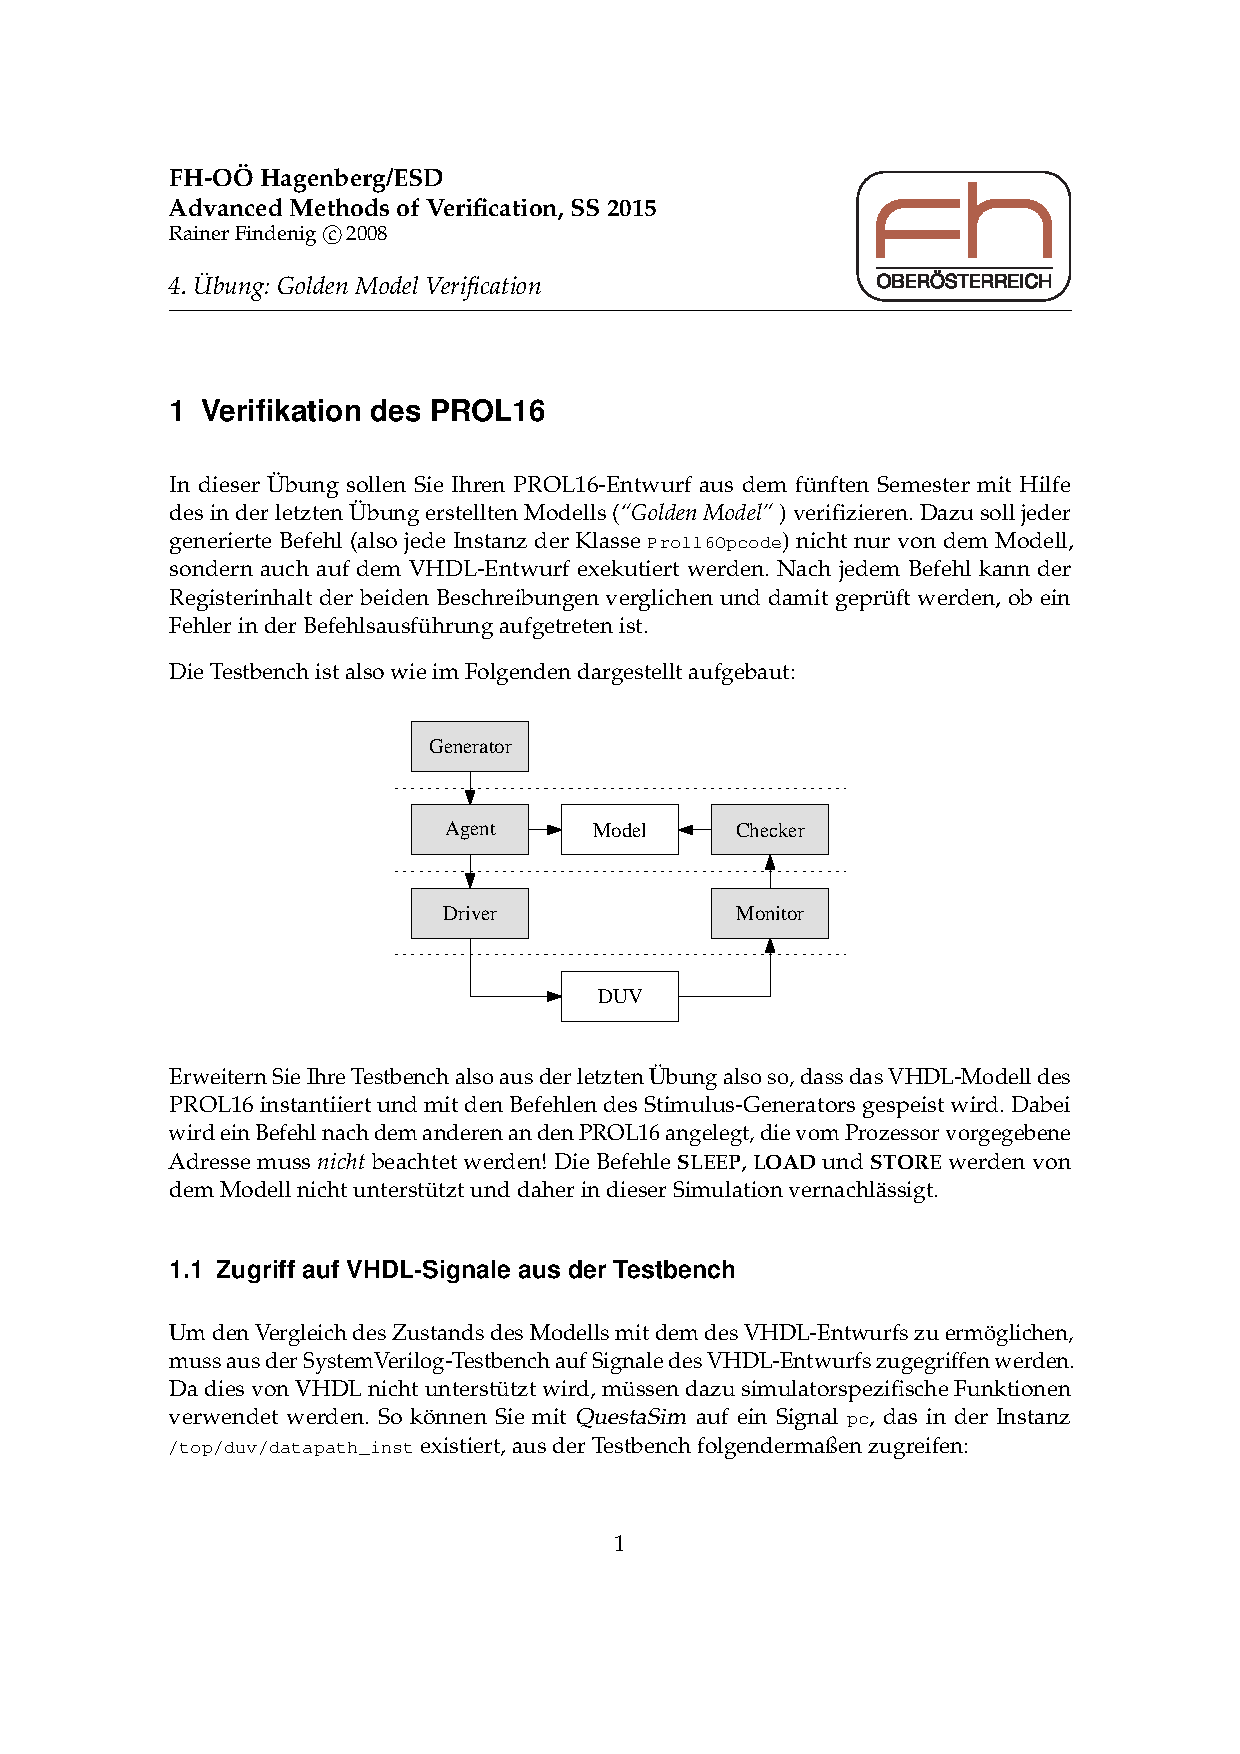
\includepdf[pages=-]{../Angabe.pdf}


\section{Testfälle}
Es wurden alle Operationen des PROL16 Befehlssatz getestet. Dabei wurden möglichst alles Register einmal verwendet. Beim Testen wurde besonders auf Carry und Zero Flag geachtet. Zusätzlich zum PROL16 Befehlsatz wurde noch ein invalider Befehl getestet und ein Move Befehl der auf ein invalides Register zugreift.
\\
Getestet und simuliert wurde auf dem Applicationserver.


\section{Source Code}

\lstinputlisting[language={verilog}]{\srcpath/pkgProl16.sv}
\lstinputlisting[language={verilog}]{\srcpath/Prol16Command.sv}
\lstinputlisting[language={verilog}]{\srcpath/Prol16Opcode.sv}
\lstinputlisting[language={verilog}]{\srcpath/Prol16State.sv}
\lstinputlisting[language={verilog}]{\srcpath/Prol16Model.sv}
\lstinputlisting[language={verilog}]{\srcpath/testProl16Model.sv}
\lstinputlisting[language={verilog}]{\srcpath/top.sv}

\lstinputlisting[language={tcl}]{\simpath/Compile.do}
\lstinputlisting[language={tcl}]{\simpath/Sim.do}

\end{document}
